\documentclass{article}

\makeatletter
\renewcommand{\fnum@figure}{Εικόνα \thefigure}
\makeatother

\usepackage[greek, english]{babel}
\usepackage{alphabeta}
\usepackage{atbegshi, picture}

% Set page size and margins
% Replace `letterpaper' with`a4paper' for UK/EU standard size
\usepackage[letterpaper,top=2cm,bottom=2cm,left=3cm,right=3cm,marginparwidth=1.75cm]{geometry}

% Useful packages
\usepackage{amsmath}
\usepackage{graphicx}
\usepackage[colorlinks=true, allcolors=blue]{hyperref}
\usepackage[utf8]{inputenc}
\usepackage{indentfirst}
\usepackage{hyperref}

\addto\captionsenglish{
  \renewcommand{\contentsname}
    {Περιεχόμενα}
}

\begin{document}

\begin{titlepage}
   \begin{center}
       \vspace*{1cm}

       \textbf{\huge Team plan v0.1}

       \vspace{0.5cm}
        Τεχνολογία Λογισμικού
            
       \vspace{1cm}

       \textbf{Κούρου Αγγελική}
       
       \begin{figure}[!htb]
        \centering
        
\includegraphics[width=0.5\textwidth]{logo.png}
        \end{figure}
        
        \vspace{0.5cm}
        
        \begin{figure}[!htb]
        \centering
        
\includegraphics[width=0.5\textwidth]{ceid.png}
        \end{figure}


       \vfill
            
       Τεχνικό Κείμενο για την Τεχνολογία Λογισμικού\\
            
       \vspace{0.5cm}
            
        \href{http://www.ceid.upatras.gr}{CEID}, \href{http://www.ece.upatras.gr}{ECE} \\
       University of Patras\\
            
   \end{center}
\end{titlepage}



\noindent Η ομάδα μας

\begin{enumerate}
  \item Βεργίνης Δημήτριος, ΑΜ: 10166634 , ECE
  \item Βλαχογιάννης Δημήτριος, ΑΜ: 1067371, CEID
  \item Κούρου Αγγελική, ΑΜ: 1067499 , CEID
  \item Μητροπούλου Αικατερίνα - Quality Manager, ΑΜ: 1067409, CEID
  \item Στεφανίδης Μάριος - Project Manager, ΑΜ:1067458, CEID
\end{enumerate}

{
  \hypersetup{linkcolor=black}
  \tableofcontents
}


\newpage


\section{Εισαγωγή}
   

 Το παρόν τεχνικό κείμενο αποτελεί τον τρόπο χειρισμού της υποχρεωτικής εργασίας στο μάθημα "Τεχνολογία Λογισμικού", άρα και την υλοποίηση του project \textbf{Medic World}. Παρακάτω θα αναλυθούν οι τρόποι και τα εργαλεία υλοποίησης της εργασίας καθώς και θα δοθούν τα διαγράμματα Gannt και Pert που αφορούν τον χρονοπρογραμματισμό της εργασίας. Κρίνεται σημαντικό να αναφερθεί πώς οι ημερομηνίες που εμφανίζονται τα διαγράμματα, αφορούν δικιές μας χρονικές εκτιμήσεις, οι οποίες αργότερα μπορεί να αλλάξουν. Οι αλλαγές θα καταγραφούν σε επόμενες εκδόσεις του τεχνικού κειμένου. 
 
 
\subsection{Ομάδα Υλοποίησης}

Η ομάδα μας αποτελείται από τα 5 άτομα που αναγράφονται παραπάνω. Μετά από σύσταση των διδασκόντων επιλέξαμε να γίνουμε μία μεικτή ομάδα συμπεριλαμβάνοντας τον Δημήτρη Βεργίνη, από το ΤΜΗΜΤΥ, τον οποίο γνωρίζουμε ως καλό developer λογισμικού στην γλώσσα που επιλέξαμε να γράψουμε τον κώδικα. Επίσης η μεταξύ μας επιθυμία για συνεργασία προέκυψε από τα εξής χαρακτηριστικά των ατόμων:
 

\begin{itemize}
  \item Καλός χρονοπρογραμματιστής, Οργανωτικός developer : Μάριος Στεφανίδης
  \item Εργατική, Γνώστης διαδραστικών τεχνολογιών : Αικατερίνα Μητροπούλου
  \item Έμπειρος developer, Γνώστης Python(αντικειμενοστραφούς προγραμματισμού) : Δημήτριος Βεργίνης
  \item Ευπροσάρμοστος στο Λογισμικό, Συγκεντρωτικές γνώσεις αντικειμενοστρέφειας : Δημήτριος Βλαχογιάννης
  \item Εργατική, Γνώστης αναγκών υλικού, Γνώσεις αντικειμενοστραφούς προγραμματισμού : Αγγελική Κούρου 
\end{itemize}


\subsection{Εργαλεία Υλοποίησης}

Έχουμε επιλέξει διάφορα εργαλεία και εφαρμογές για την υλοποίηση της εν λόγω εργασίας. Παρακάτω αναλύονται οι ανάγκες που πρέπει να καλυφθούν και ποιές εφαρμογές επιλέχθηκαν.


\begin{itemize}
    \item Προγραμματισμός σε Puthon : Pycharm, Vscode
    \item Διαγράμματα Gannt : \href{https://www.monday.com}{Monday}
    \item Διαγράμματα Pert : \href{https://lucid.app}{Lucidchart}
    \item Επεξεργασία Τεχνικών Κειμένων : \href{https://www.overleaf.com}{Overleaf}
    \item Mock-up Screens : \href{https://www.mockflow.com/}{Mockflow}, \href{https://www.figma.com}{Figma}
    \item Αποθήκευση, Επεξεργασία Τεχνικών Κειμένων : \href{https://github.com/}{Github}
\end{itemize}
 

\subsection{Μέθοδος Ανάπτυξης Λογισμικού}

Ύστερα από συγκεντρωτική ψηφοφορία, επιλέχθηκε η μέθοδος ανάπτυξης λογισμικού \textbf{Scrum} για την υλοποίηση αυτής της εργασίας. Θεωρήθηκε ταιριαστή αυτή η μέθοδος για διάφορους λόγους. Πρώτον, στα πλαίσια ενός εξαμήνου, για να ολοκληρωθούν 6 παραδοτέα θα χρειαστούν sprint cycles για την ολοκλήρωση του project. Στο τέλος κάθε κύκλου εργασίας, θα αξιολογείται η πρόοδος της ομάδας από τους "πελάτες" (διδάσκοντες). Δεύτερον, με πλήθος 5 ατόμων σε μία ομάδα χρειάζεται ο ηγετικός ρόλος του \textbf{Scrum Master} ή \textbf{Project Manager} για να οργανώσει την δουλειά και να ελέγξει τα μέλη. Ακόμα το γεγονός πως η ομάδα παρουσιάζει ετερογένεια, όσον αφορά την σχολή φοίτησης και υπάρχουν διαφορές στις ώρες εργασίας, συνιστά έναν ακόμα λόγο να υπάρχει κάποιος υπεύθυνος που θα συνεννοείται με όλους τους developers ώστε να έρθει η εργασία είς πέρας. Έτσι επιλέχθηκε το \textbf{Scrum} ως ιδανικός τρόπος ανάπτυξης λογισμικού.

\newpage

\section{Διαγράμματα χρονοπρογραμματισμού}



\subsection{Διαγράμματα Gannt}

Τα παρακάτω διαγράμματα χρονοπρογραμματισμού δημιουργήθηκαν βάσει των ζητούμενων παραδοτέων τεχνικών κειμένων, με προσωπική εκτίμηση της χρονικής διάρκειας κάθε παραδοτέου. Έγιναν με την βοήθεια του online εργαλείου \href{https://www.monday.com}{Monday}

\vspace{0.3cm}

\begin{figure}[!htb]
\centering
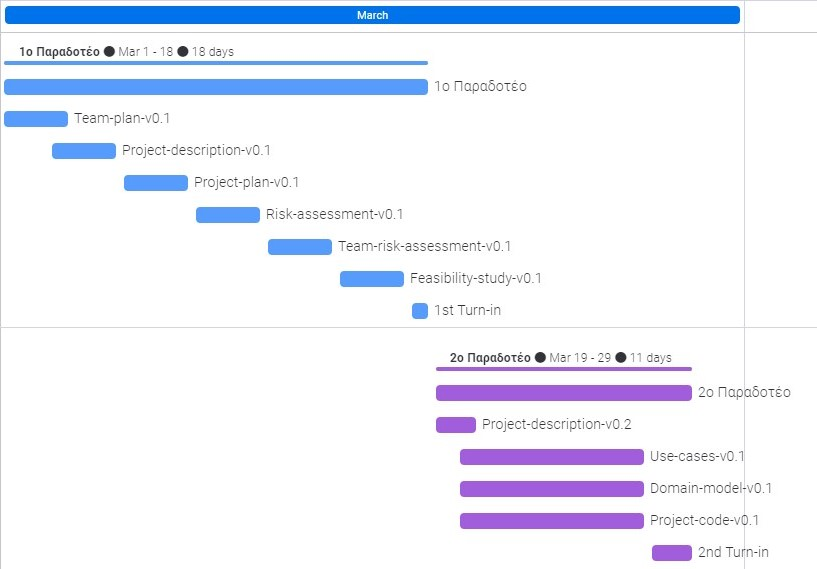
\includegraphics[width=0.9\textwidth]{Team-plan-Gannt-1.jpg}
\caption{\label{fig:log in page} Παραδοτέα 1, 2}
\end{figure}
 
 
\begin{figure}[!htb]
\centering
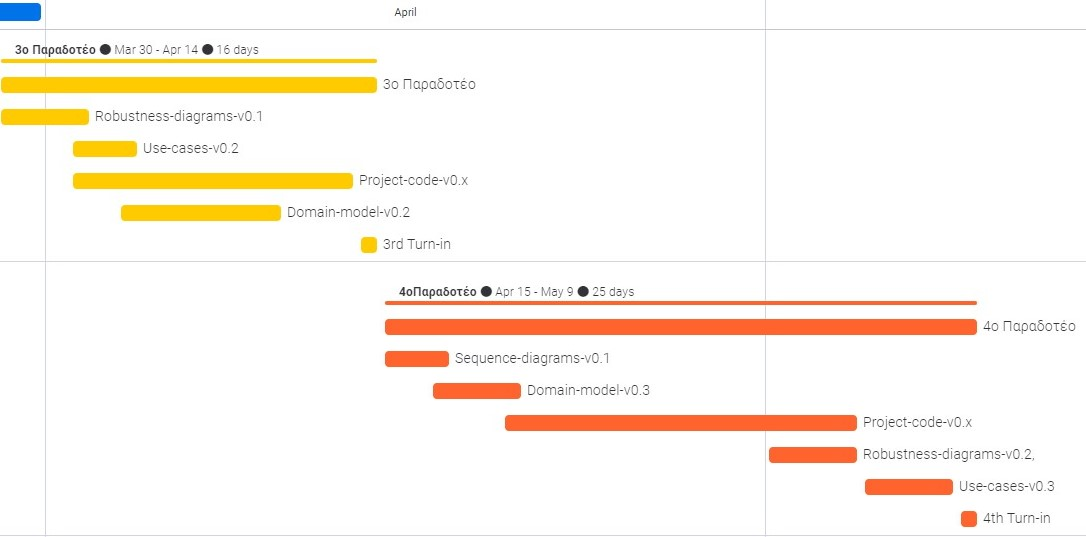
\includegraphics[width=1.0\textwidth]{Team-plan-Gannt-2.jpg}
\caption{\label{fig:log in page} Παραδοτέα 3, 4}
\end{figure}


\begin{figure}[!htb]
\centering
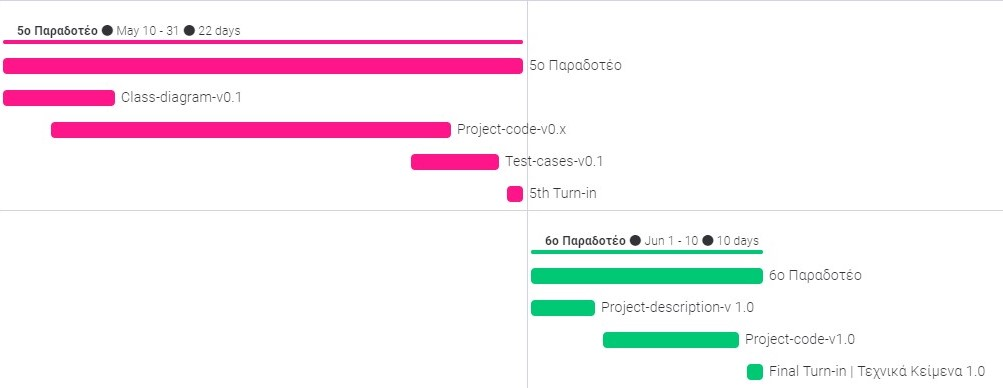
\includegraphics[width=1.0\textwidth]{Team-plan-Gannt-3.jpg}
\caption{\label{fig:log in page} Παραδοτέα 5, 6}
\end{figure}



\subsection{Διαγράμματα Pert}
Τα Pert flowcharts που αφορούν τα παραδοτέα της εργασίας, ξανά με προσωπική εκτίμηση των χρονικών περιόδων είναι παρουσιασμένα παρακάτω. Έγιναν με την βοήθεια του online εργαλείου \href{https://lucid.app}{Lucidchart}. Για περαιτέρω βοήθεια στην κατανόηση πρέπει να γίνουν οι εξής διευκρινίσεις:

\begin{itemize}
  \item Με μαύρο βελος συμβολίζονται τα τεχνικά κείμενα που θα μπορούσαν να συγγραφούν παράλληλα και δεν σχετίζονται αυστηρά ώστε η συγγραφή του ενός να είναι μη πραγματοποιήσιμη χωρίς το άλλο.
  \item Με κόκκινο βέλος συμβολίζονται είτε τα υποχρεωτικά παραδοτέα κάθε εργασίας, είτε η σύνδεση έκδοσης ενός τεχνικού κειμένου με ένα άλλο κείμενο παραδοθέν σε προηγούμενη έκδοση της εργασίας.
  \item Οι κίτρινοι ρόμβοι συμβολίζουν τα milestones, επομένως στην προκειμένη περίπτωση τις ολοκληρωμένες παραδόσεις της εργασίας.
\end{itemize}

Σημαντικό κρίνεται επίσης να σημειωθεί, ότι στο τελευταίο διάγραμμα για να αποφυγεί η δυσκολία κατανόησης με ένα milestone έχουν αποτυπωθεί και οι 5 προηγούμενες επιτυχημένες παραδόσεις του project ως ένα milestone. Συγκεντρωτικά οι 5 προηγούμενες εκδόσεις της εργασίας αποτελούν ένα milestone για την τελική μορφή της εργασίας.

\newpage

\begin{figure}[!htb]
\centering
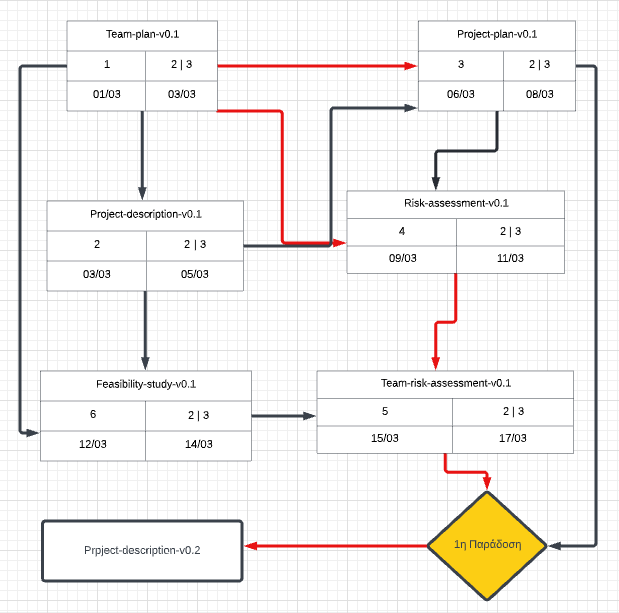
\includegraphics[width=0.6\textwidth]{Team-plan-Pert-1.png}
\caption{\label{fig:log in page}Διάγραμμα Pert  1}
\end{figure}
 
 
\begin{figure}[!htb]
\centering
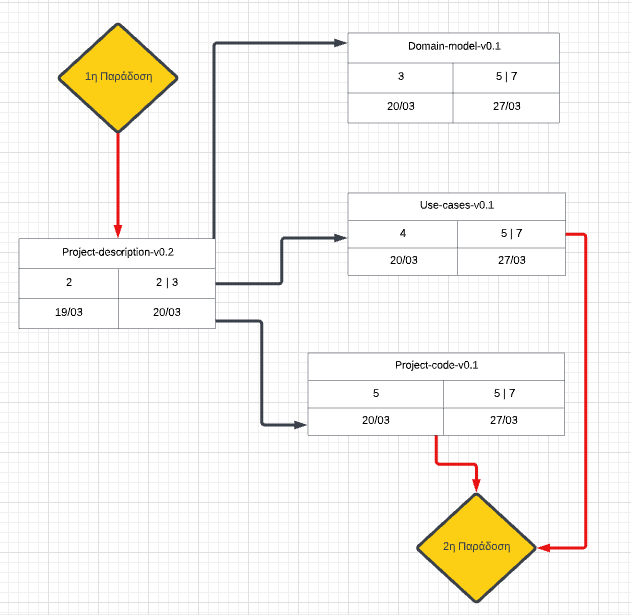
\includegraphics[width=0.6\textwidth]{Team-plan-Pert-2.png}
\caption{\label{fig:log in page}Διάγραμμα Pert  2}
\end{figure}


\begin{figure}[!htb]
\centering
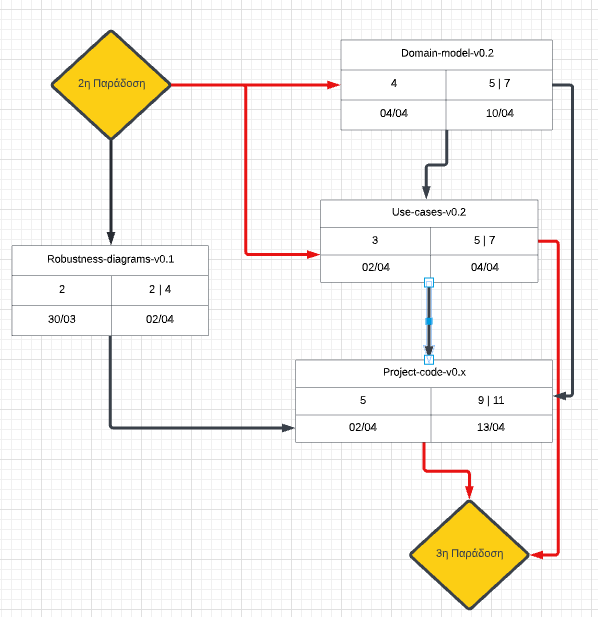
\includegraphics[width=0.6\textwidth]{Team-plan-Pert-3.png}
\caption{\label{fig:log in page}Διάγραμμα Pert  3}
\end{figure}

\begin{figure}[!htb]
\centering
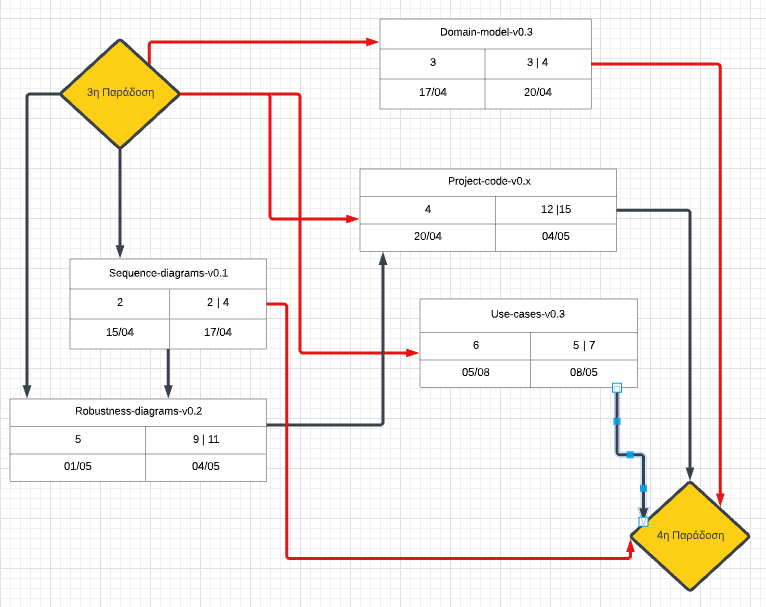
\includegraphics[width=0.8\textwidth]{Team-plan-Pert-4.png}
\caption{\label{fig:log in page}Διάγραμμα Pert  4}
\end{figure}

\begin{figure}[!htb]
\centering
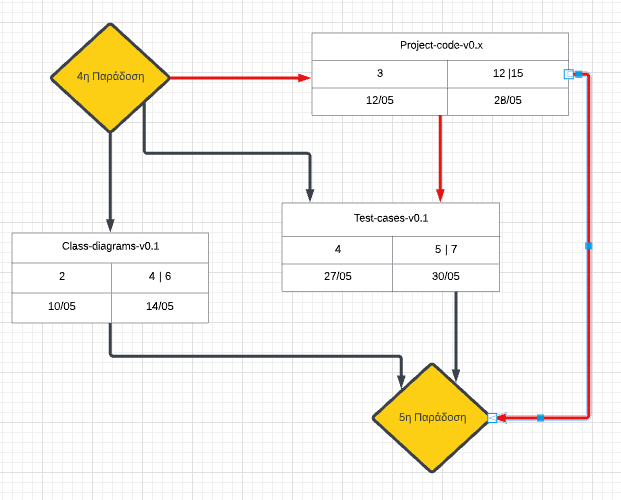
\includegraphics[width=0.8\textwidth]{Team-plan-Pert-5.png}
\caption{\label{fig:log in page}Διάγραμμα Pert  5}
\end{figure}
\begin{figure}[!htb]
\centering
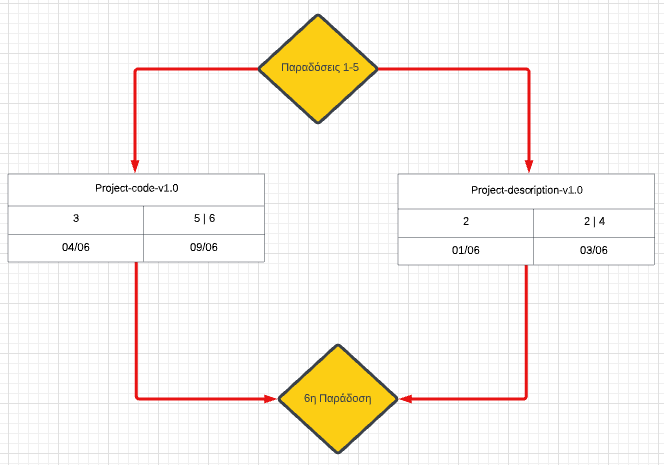
\includegraphics[width=0.8\textwidth]{Team-plan-Pert-6.png}
\caption{\label{fig:log in page}Διάγραμμα Pert 6}
\end{figure}


\newpage


\end{document}
